\documentclass[10pt]{article}
\usepackage{amsmath,textcomp,amssymb,geometry,graphicx,enumerate,tikz,algorithm,algpseudocode,pifont}
\usetikzlibrary{calc}
\usetikzlibrary{datavisualization}
\usetikzlibrary{datavisualization.formats.functions}


\textheight=9in
\textwidth=7in
\topmargin=-.75in
\oddsidemargin=-0.25in
\evensidemargin=-0.25in

\usepackage{listings}
\lstnewenvironment{codeblock}
    {\lstset{language=Python,
      showspaces=false,
      showtabs=false,
      breaklines=true,
      mathescape=true,
      showstringspaces=false,
      breakatwhitespace=true,
      commentstyle=\textit,
      keywordstyle=\textbf,
      basicstyle=\ttfamily,
      escapechar=`,
      moredelim={**[is][{\color{RoyalBlue}}]{\^^M\\beginsol}{\^^M\\endsol}},
      moredelim={[is][{\color{RoyalBlue}}]{\^^M\\beginexp}{\^^M\\endexp}},
    }}
    {}

\newcommand{\bigo}{\mathcal{O}}


\begin{document}
\section*{03/30/2016}
\subsection*{Neural Networks}
\begin{itemize}
	\item Can do both classification and regression.
	\begin{center}
		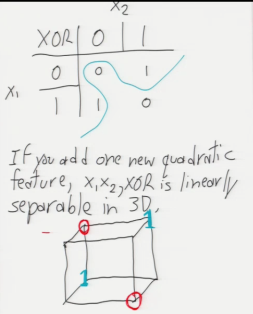
\includegraphics[scale=0.5]{../images/xorseparable}
		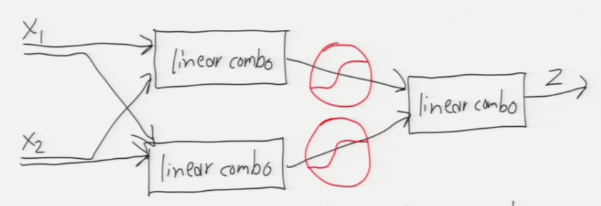
\includegraphics[scale=0.5]{../images/simplenet}
	\end{center}
	\item A linear combination of a linear combination is a linear combination... only works for linearly separable samples.
	\begin{center}
		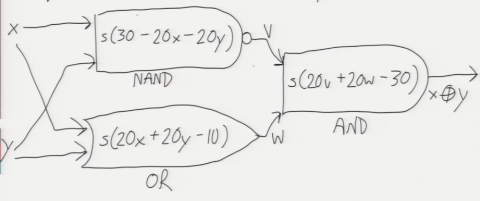
\includegraphics[scale=0.5]{../images/xornet}
	\end{center}
\end{itemize}

\subsubsection*{Network with 1 Hidden Layer}
\begin{itemize}
	\item Input layer: $x_{1}, \dots, x_{d}; \ x_{d+1} = 1$
	\item Hidden units: $h_{1}, \dots, h_{m}; \ h_{m+1} = 1$
	\item Output layer: $z_{1}, \dots, z_{k}$
	\item Layer 1 weights: $m \ \text{x} \ (d+1)$ matrix $V$ $V_{i}$ is row $i$
	\item Layer 2 weights: $k \ \text{x} \ (m+1)$ matrix $W$ $W_{i}$ is row $i$
	\item Recall logistic function $s(\gamma) = \frac{1}{1 + e^{-\gamma}}$. Other nonlinear functions can be used.
	\item For vector $v$, $s(v) = \begin{bmatrix}
									s(v_{1})\\
									s(v_{2})\\
									\vdots\\
									s(v_{n})\\
								\end{bmatrix}$
	\begin{center}
		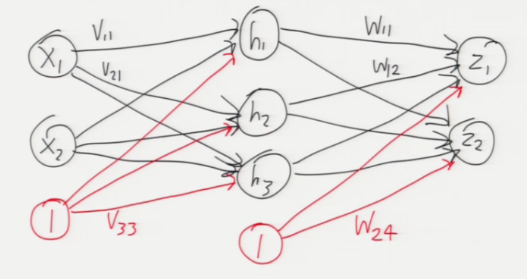
\includegraphics[scale=0.5]{../images/nn}
	\end{center}
	\item $h_{i} = s(\sum_{j=1}^{n} V_{ij}x_{j})$, in short, $h = s(Vx)$.
	\item $z = s(Wh) = s(Ws_{1}(Vx))$ the one on the $s$ means you have to add a 1 to end of vector before multiplication.
\end{itemize}

\subsubsection*{Training}
\begin{itemize}
	\item Usually stochastic or batch gradient descent.
	\item Pick loss function $L(z, y), \ z=\text{predictions}, \ y=\text{true (values often a vector)}$ e.g. $L(z, y) = |z - y|^{2}$.
	\item Cost function is $J(h) = \sum_{i=1}^{n} L(h(X_{i}, Y_{i}))$. Start with random weights.
	\item Usually there are many local minima!
	\item Rewrite all the weights in $V$ and $W$ as a vector $w$.
\begin{codeblock}
    Batch gradient descent:
	    $w \leftarrow$ vector of (small) random weights
	    repeat:
	        $w \leftarrow w - \epsilon \nabla J(w)$
\end{codeblock}
	\item Hard part is computing $\nabla J(w)$.
	\item Naive gradient computation: $\bigo (\text{units x edges})$ time.
	\item Back-propagation: $\bigo (\text{edges})$ time.
\end{itemize}

\subsubsection*{Computing Gradients for Arithmetic Expressions}
	\begin{center}
		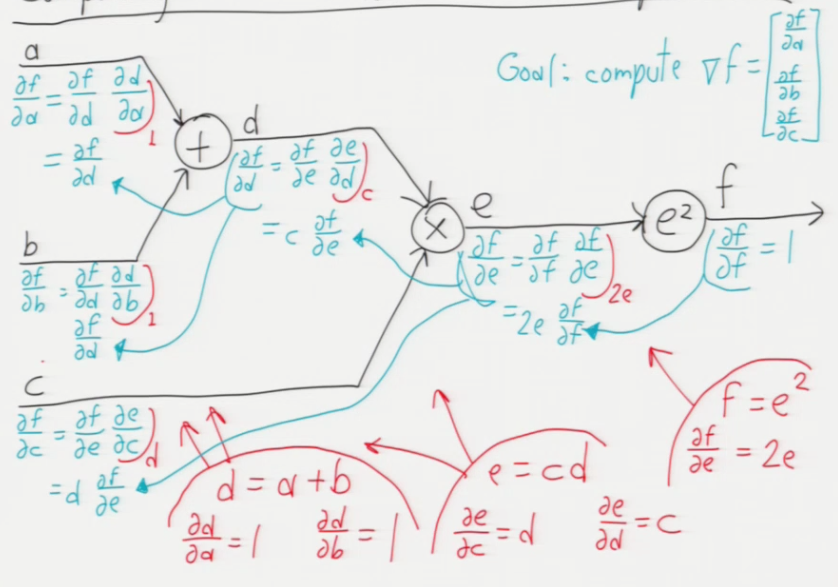
\includegraphics[scale=0.3]{../images/backprop}
	\end{center}
\begin{itemize}
	\item Each value $z$ gives partial derivative of the form,
		\begin{align*}
			\frac{\partial f}{\partial z} = \frac{\partial f}{\partial n} \frac{\partial n}{\partial z}\\ 
		\end{align*}
	\item Can always compute $\frac{\partial n}{\partial z}$ in forward pass.
	\item Compute $\frac{\partial f}{\partial n}$ during backward pass \underline{after} forward pass.
	\item This is "back-propagation."
	\begin{center}
		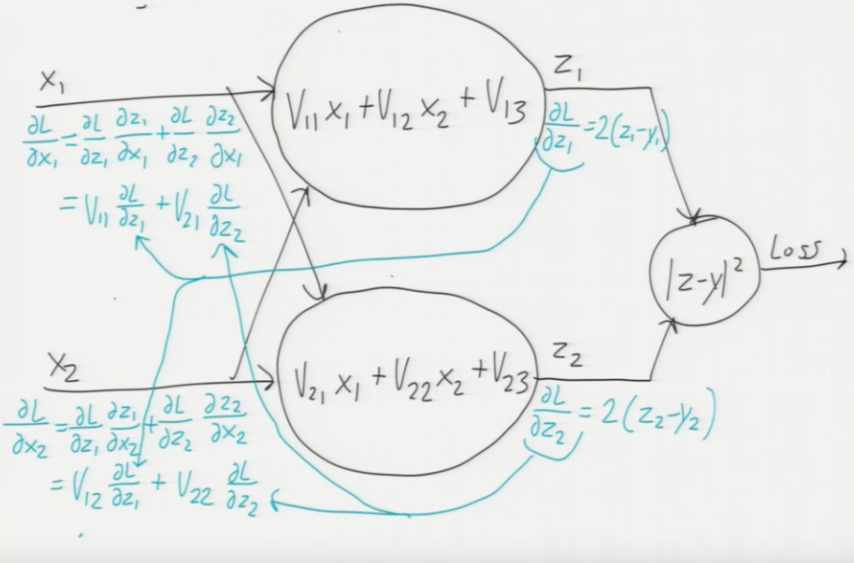
\includegraphics[scale=0.4]{../images/net}
	\end{center}
	\item Algorithm doesn't work if there's cycles.
\end{itemize}

\subsubsection*{The Back-propagation Algorithm}
\begin{itemize}
	\item Recall $s'(\gamma) = s(\gamma)(1-s(\gamma))$
	\item $h_{i} = s(V_{i} \cdot x)$, so $\nabla_{v_{i}} h_{i} = s'(V_{i}\cdot x)x$
		\begin{center}
			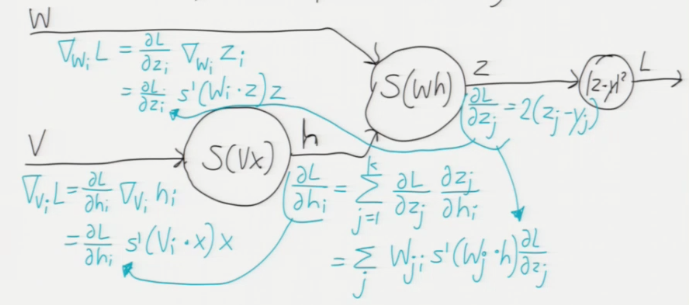
\includegraphics[scale=0.5]{../images/neurals.png}
		\end{center}
\end{itemize}




\end{document}